\documentclass[11pt,a4paper,english,oneside, pdf]{article}
\usepackage[margin=2.5cm]{geometry}
\usepackage[utf8]{inputenc} %Permite introducir directamente acentos: á en lugar de \'a etc.
\usepackage{mathtools}
\usepackage{palatino}
\usepackage{graphicx}
\usepackage{hyperref}
\usepackage{xcolor}
\usepackage{tikz}
\usetikzlibrary{shapes.geometric, arrows}


\title{BACoN analysis RUN 3}
\author{Carmen Romo Luque}

\graphicspath{{/Users/romoluque_c/Repositories/BACON_romo/analysis_documentation_run3/images/}}

\begin{document}
	\maketitle
	
	
	\tableofcontents
	
	
	\clearpage
	
	\section{Introduction}	 
	 The BACoN detector is designed to investigate the scintillation properties of liquid argon when doped with xenon. The setup consists of a 100-liter cylindrical cryostat filled with liquid argon, featuring a single upward-facing PMT mounted at the bottom and four rows of three equidistantly spaced SiPMs. Each SiPM row is separated by 10 cm from the next one. On top of the cylinder, an Americium source is placed, emitting gammas and alphas that interact with the liquid, producing scintillation light. The first row of SiPMs is positioned close to the decay source and serves as the trigger system when all of them detect at least one photoelectron. These three SiPMs are collimated to prevent potential saturation effects.
	 
	 %\begin{figure}[!h]
	 %	\begin{center}
	 %		\includegraphics[width=9cm]{BACoN_picture_run2}
	 %		\caption{New setup of the BACoN detector. The PMT is placed at the bottom of the chamber and 4 rows of SiPMs arranged around 10 cm apart, facing the americium source.}
	 %		\label{fig:BACoN_picture_run2}
	 %	\end{center}
	 %\end{figure}
	 
	 The cryostat's liquid argon level is continuously monitored by measuring its weight. Additionally, the argon undergoes purification via a SAES PS4-MT3/15-R getter, which removes impurities such as H$_2$0, CO, CO$_2$, N$_2$, H$_2$, CH$_4$, reducing their concentrations to less than 1 part per billion (PPB) prior to liquefaction.
	 
	 
	 \clearpage
	 
	 \section{Nomenclature}
	 
	 \begin{itemize}
	 	\item \textbf{Channel:}  individual readout or signal processing pathway associated with a single detector. In BACoN each detector (SiPM or PMT) corresponds to a channel. In LEGEND-200 for example, 9 SiPMs make one channel.
	 	\begin{itemize}
	 		\item Channels 0-8: non-trigger SiPMs.
	 		\item Channels 9-11: trigger/source SiPMs.
	 		\item Channel 12: PMT.
	 	\end{itemize}
	 	
	 	\item \textbf{Waveform:} time-dependent electrical signal produced by the detector in response to photon interactions.
	 	
	 	\item \textbf{Event:} coincident set of signals corresponding to a physical interaction that occurs within a defined time window, recorded across multiple SiPM and PMT channels. Each event comprises the waveforms from all SiPM and PMT channels that capture the interaction, allowing the reconstruction of the event's spatial, temporal, and energy characteristics.
	 	
	 	\item \textbf{Run:} continuous set of data that start the same day and are collected over a single or subsequent days (in the case of BACoN), including multiple files that sequentially store the recorded information. No hardware changes are introduced within a run.
	 	
	 	\item \textbf{Period:} set of subsequent runs with the same hardware conditions. For example a new period should start when adding a different amount of xenon doping.
	 	
	 	\item \textbf{Hit:} represents the timestamp (or sample number), energy (in ADC or PE) and channel of each individual peak of photons.
	 \end{itemize}
	  
	 
	
	\clearpage
	
	\section{Data analysis flow}
	\label{data_analysis_flow_sec}
	
	Steps:
	
	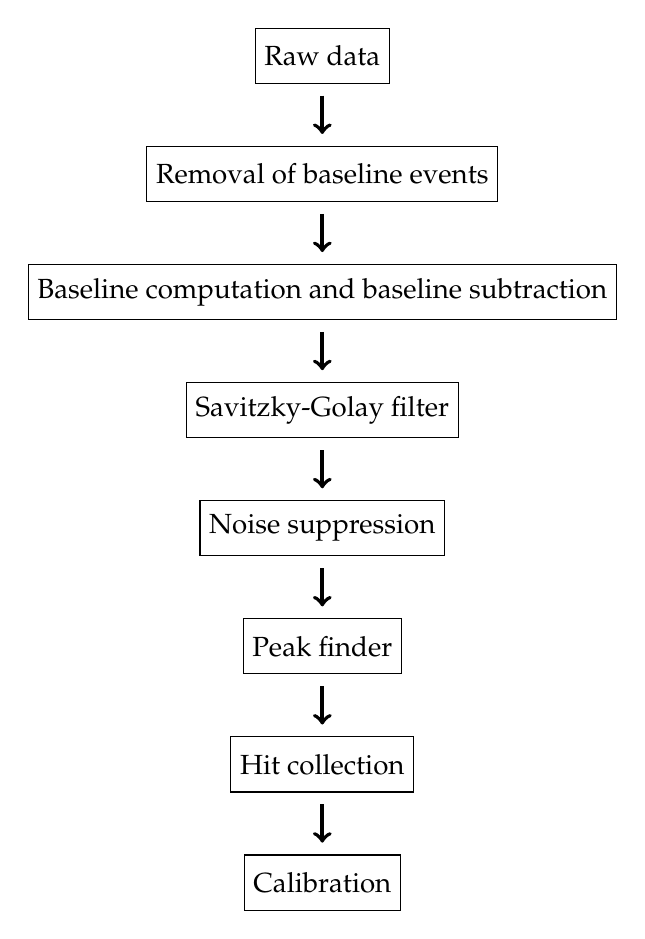
\begin{tikzpicture}[node distance=1.5cm]
		% Define styles for the blocks and arrows
		\tikzstyle{block} = [rectangle, draw, text centered, minimum height=0.7cm]
		%\tikzstyle{arrow} = [thick,->,>=stealth]
		\tikzstyle{arrow} = [thick,->,>=to, shorten >=1.5mm, shorten <=1.5mm, line width=0.5mm]
		
		
		% Define the nodes (blocks)
		\node (raw) [block] {Raw data};
		\node (removal) [block, below of=raw] {Removal of baseline events};
		\node (computation) [block, below of=removal] {Baseline computation and baseline subtraction};
		\node (filter) [block, below of=computation] {Savitzky-Golay filter};
		\node (noise) [block, below of=filter] {Noise suppression};
		\node (peakf) [block, below of=noise] {Peak finder};
		\node (hits) [block, below of=peakf] {Hit collection};
		\node (calibration) [block, below of=hits] {Calibration};

		% Draw arrows between the blocks
		\draw [arrow] (raw) -- (removal);
		\draw [arrow] (removal) -- (computation);
		\draw [arrow] (computation) -- (filter);
		\draw [arrow] (filter) -- (noise);
		\draw [arrow] (noise) -- (peakf);
		\draw [arrow] (peakf) -- (hits);
		\draw [arrow] (hits) -- (calibration);
	\end{tikzpicture}
	
	\subsection{Raw data}
	\label{raw_data_sec}
	
	In BACoN, a new event begins when the three trigger SiPMs detect at least one photoelectron each. Once this condition is met, data from all the sensors are recorded. The raw data are saved in ROOT files. Figure \ref{fig:rawdata} shows an example of the individual signals for an event: the top panel shows signals from all the SiPMs (ordered according to their geometrical location, with channels 9, 10 and 11 being the trigger SiPMs), and the bottom panel shows the signal from the PMT (channel 12). In each event, the three trigger SiPMs always register a signal (which triggers the event), while most of the other channels do not detect light. Occasionally, one or more channels will show peaks corresponding to gamma interactions in the liquid argon. For example, the plot for channel 8 shows a single-photon peak. The signal of the trigger SiPMs is inverted due to the amplifier, since the discriminator for the trigger system only accepts negative signals.
	
		\begin{figure}[!h]
			\begin{center}
				\includegraphics[width=\textwidth]{rawdata_sipms.pdf}
				
				\vspace{0.6cm}
				\includegraphics[width=0.5\textwidth]{rawdata_pmt.pdf}
				\caption{Example of an event recorded in BACoN. The three plots in the first row correspond to the trigger SiPMs, which always register a signal, as this is the condition for an event to begin. The nine plots in the following rows show signals from the non-trigger SiPMs: channels 0, 1, and 2 are in the bottom row; channels 3, 4, and 5 are in the middle row; and channels 6, 7, and 8 are in the top row, closer to the trigger SiPMs. The distance between rows is approximately 15 cm. The plot at the bottom shows the PMT (channel 12) signal, which is also inverted, as is the case for the trigger SiPMs.}
				\label{fig:rawdata}
			\end{center}
		\end{figure}
		
	
	\subsection{Baseline}
	\label{baseline_sec}
	
	
	The first check of the SiPMs and the PMT data is the baseline. The baseline can be computed using either the mean or the mode of the entire waveform, or by selecting a specific range. Since the trigger time in BACoN is close to 1500 ns, we use the first 1300 ns of the waveform to avoid including peaks in the chosen region, as shown in blue in Figure \ref{fig:baseline_region}. Figure \ref{fig:baselines} shows the baseline over time for several runs taken in September. The baseline appears to be decreasing over time, and the deviation from the mean is higher in the trigger SiPMs compared to the normal SiPMs.
	
	\begin{figure}[!h]
		\begin{center}
			\includegraphics[width=0.8\textwidth]{Baseline_region.pdf}
			\caption{Multiple waveforms from a trigger SiPM showing the trigger time. The region before the trigger time, shown in blue, is used to compute the baseline in order to minimize the influence of any peaks that could interfere with the baseline calculation.}
			\label{fig:baseline_region}
		\end{center}
	\end{figure}
	
	
	\begin{figure}[!h]
		\begin{center}
			\includegraphics[width=0.49\textwidth]{baselines_rel1.pdf}
			\includegraphics[width=0.477\textwidth]{baselines_rel2.pdf}
			\caption{.}
			\label{fig:baselines}
			\end{center}
	\end{figure}
	
	
	\begin{figure}[!h]
		\begin{center}
			\includegraphics[width=\textwidth]{baselines_rel1_norm_ch.pdf}
			\caption{.}
			\label{fig:baselines2}
		\end{center}
	\end{figure}

	\begin{figure}[!h]
		\begin{center}
			\includegraphics[width=\textwidth]{baselines_rel1_trigg_ch.pdf}
			\caption{.}
			\label{fig:baselines3}
		\end{center}
	\end{figure}
	
	
	
	\subsubsection{Baseline at beginning and end of waveform}
	
	
	\subsubsection{Baseline subtraction}
	
	
	
	\begin{figure}[!h]
		\begin{center}
			\includegraphics[width=\textwidth]{Baseline_subtraction_wf.pdf}
			\caption{.}
			\label{fig:bsl_subt_wf}
		\end{center}
	\end{figure}
	
	
	
	\subsection{Convolution and baseline subtraction for trigger SiPMs}
	\label{conv_and_bsl_subt_sec}
	
	
	
	\subsection{Savitzky-Golay filter}
	\label{sg_filter_sec}
	
	First, it is necessary to apply a threshold to reject noise. However, noise counts could be mistaken for signal if they exceed the selected threshold. To mitigate this issue, we employ the Savitzky-Golay (SG) filter. This filter effectively removes noise from signals while preserving important features such as peaks and valleys. It is particularly useful when dealing with noisy data, enabling clearer analysis of the underlying signal.
	
	\begin{figure}[!h]
		\begin{center}
			\includegraphics[width=11cm]{SG_filter_wf_close.pdf}
			\caption{Subtracted waveform (black) and waveform (salmon) after applying the Savitzky-Golay filter.}
			\label{fig:SG_waveform}
		\end{center}
	\end{figure}
	
	Figure \ref{fig:SG_waveform} shows a subtracted waveform and the result after filtering using the Savitzky-Golay (SG) filter. As depicted in Figure \ref{fig:SG_waveform_thr}, with this filter, we can ensure that no counts from the baseline exceed the desired threshold.
	
	\begin{figure}[!h]
		\begin{center}
			\includegraphics[width=16cm]{SG_waveform_wl30ns_thr_points.pdf}
			\caption{Left: subtracted waveform; right: subtracted and filtered waveform. The points above the chosen threshold (30 ADC, for example) have been plotted to illustrate that after filtering, no points from the baseline are present that could lead to a misinterpretation of the signal.}
			\label{fig:SG_waveform_thr}
		\end{center}
	\end{figure}
	
	One consideration when employing this method is that the heights of the peaks after filtering will be slightly reduced. Therefore, to address such variations, SiPM calibration should also be conducted using this method.
	
	\subsubsection{Comparison between SG and Wiener filter}
	
	
	\subsection{Noise suppression}
	\label{noise_suppression_sec}
	
	\subsubsection{Threshold applied to the SiPMs.}
	
	
	\subsection{Peak finder}
	\label{peak_finder_sec}
	
	\subsubsection{Single PE shape}
	\begin{itemize}
		\item Averaged waveform
		\item Fit wfs to a Landau distribution
	\end{itemize}
	
	\subsubsection{Distance between peaks in non-trigger SiPMs}

	\subsubsection{Distance between peaks in trigger SiPMs}	
	
	\subsubsection{Second peaks analysis method}
	
	\subsubsection{Trigger time}
	
	\subsection{Hit collection and time distribution}
	\label{hits_sec}
	
	
	
	\subsection{Sum of the 1PE waveforms}
	\label{sum_wfs_sec}
	
	
	
	\subsection{SiPM calibration}
	\label{calibration_sec}
	
	Maintaining the optimal performance of sensors in the BACoN system is crucial for accurate data collection, enabling the detection of variations in light levels within the detector. For this, periodic calibrations of the SiPMs are conducted to verify their proper functioning and stability. Despite employing the same sensor model across all SiPMs, variations in analog-to-digital conversion (ADC) counts in response to identical light inputs are inevitable. Hence, regular calibration of the SiPMs at the single photon level is imperative to standardize their responses and assess their long-term stability.
	
	Ideally, a chamber should be equipped with LEDs for performing regular calibrations during data collection. That would allow us to monitor gain variations over time at a controlled light intensity, particularly important for long-term data acquisitions lasting several months or few years. Additionally, since we operate at low temperatures, the gains of the SiPMs won't match those obtained during black box calibration. However, in the absence of LEDs, we can still utilize low-light data for similar calibrations, though it's important to note that the values may differ.
	
	Due to the low temperature required to maintain argon in its liquid state within the BACoN detector, the bias voltage of the SiPMs needs to be reduced. This compensates for the decrease in breakdown voltage of the silicon diodes within the SiPM structure under reduced thermal conditions. At lower temperatures, the breakdown voltage tends to increase, meaning that the same bias voltage applied at room temperature could potentially cause the SiPMs to operate in a regime where the breakdown voltage is exceeded. This can lead to excess dark count rate and decreased performance. Therefore, reducing the bias voltage when operating SiPMs at lower temperatures helps ensure that they remain within their optimal operating conditions and maintain stable performance. That's the reason why the gains of the SiPMs inside the chamber are higher even at a lower bias voltage.
	
	
	First, we subtract the baseline of the waveform, which allows us to obtain the absolute height of the peaks. The baseline subtraction procedure can be performed by computing either the mean value or the mode of the entire waveform or just a certain range. 
	Then, we compute the single photon spectra by getting the height of the peaks at the trigger region. 
	
	
	Subsequently, a histogram is generated displaying the heights of the peaks in the trigger window, allowing for the identification of individual single photoelectron peaks. First, a poisson distribution of a certain number of gaussians is perfomed in order to extract the mean position of each photoelectron peak. The gain is then calculated from the spectrum using the distance between the pedestal peak and those for 1, 2, ...  photoelectrons.
	
	
	Then, the linear regression of the mean achieved enables the extraction of the conversion factor between ADC and photoelectrons. With these values, the response across all channels can be standardize.
	
	
	
	\clearpage
	
	\section{Pile-up events}
	
	Pile-up occurs when multiple photons arrive to a SiPM within a very short time window, resulting in overlapping signals that the detector cannot distinguish as separate events.
	
	In BACoN, we have observed that, occasionally, there are pile-up signals and these are not straight-forward to deconvolve. To understand these types of events, we should first clarify what a single photoelectron signal looks like. The left side of Figure \ref{fig:1PE_signal} shows multiple single PE waveforms for channel 8 in blue, with their average amplitude in black. The shape of the single PE signal follows a Landau distribution, as seen in the fit on the right side of Figure \ref{fig:1PE_signal}.
	
	\begin{figure}[!h]
		\begin{center}
			\includegraphics[width=0.49\textwidth]{images/1PE_wfs_and_average_ch8.pdf}
			\includegraphics[width=0.46\textwidth]{images/averaged_single_PE_wfs_fit_Landau.pdf}
			\caption{Left: superposition of 100 single-photon waveforms for a selected channel (channel 8) in blue, with the averaged waveform in black. Right: fit of the averaged waveform to a Landau distribution.}
			\label{fig:1PE_signal}
		\end{center}
	\end{figure}
	
	The width of the single PE peak depends on the amplitude chosen as the reference. In Figure \ref{fig:width_1PE_signal}, we can see the averaged single PE waveform along with the crossing points at different threshold amplitudes. The red case corresponds to a threshold of 50 ADC, while the green case corresponds to a threshold of 80 ADC.
	
	\begin{figure}[!h]
		\begin{center}
			\includegraphics[width=0.49\textwidth]{images/width_single_PE_peak_ch8.pdf}
			\caption{Single photon averaged waveform with the crossing points at 50 ADC (red) and 80 ADC (green).}
			\label{fig:width_1PE_signal}
		\end{center}
	\end{figure}
	
	The left side of Figure \ref{fig:width_1_and_2_PE} shows the averaged 1PE and 2PE waveforms after smoothing with the Savitzky-Golay filter. The different widths corresponding to the different numbers of photoelectrons can be seen. On the right, the histogram of the widths for multiple waveforms in each case is shown. The mean 1PE widths are 118 ns and 72 ns for threshold values of 50 and 80 ADC, respectively, while the mean 2PE widths are 198 ns and 149 ns for thresholds of 50 and 80 ADC, respectively.
	
	\begin{figure}[!h]
		\begin{center}
			\includegraphics[width=0.49\textwidth]{images/width_1_and_2_PE_peak_sg.pdf}
			\includegraphics[width=0.46\textwidth]{images/width_1_and_2_PE_peak_comparison_hist_norm_ch8.pdf}
			\caption{Left: averaged waveforms for 1 and 2 PEs after filtering with the Savitzky-Golay filter, with the corresponding crossing points at 50 ADC (red) and 80 ADC (green). Right: histogram of the 1 and 2 PE widths for the two different thresholds (50 and 80 ADC) using SG-filtered waveforms from a selected data file.}
			\label{fig:width_1_and_2_PE}
		\end{center}
	\end{figure}
	
	These numbers are crucial for the input parameters in our peak-finding algorithm. In the past, we used a minimum distance between peaks of 30 ns, which is very small compared to the results shown here. The individual events in Figure \ref{fig:pile_up_evts} demonstrate that the minimum distance we should require in our analysis is much greater than 30 ns. The two plots on top correspond to events where no pile-up is present, but instead, fluctuations in the noise. If the wrong minimum distance between peaks and threshold amplitude are chosen, the second peak in the event on the left and the first peak in the event on the right can be incorrectly labeled as valid peaks when they are not. In contrast, the two plots below show pile-up events that we want to keep and attempt to deconvolve to extract their amplitude. These events have a distance between peaks that is always above 100 ns. For these reasons, a threshold of 80 ADC in amplitude was chosen to reject the noise, and a minimum distance of 100 ns between peaks (corresponding to 50 time samples) was set.
	
	\begin{figure}[!h]
		\begin{center}
			\includegraphics[width=0.49\textwidth]{images/pile_up_evt_329_ch8.pdf}
			\includegraphics[width=0.49\textwidth]{images/pile_up_evt_1053_ch8.pdf}
			\includegraphics[width=0.49\textwidth]{images/pile_up_evt_1037_ch8.pdf}
			\includegraphics[width=0.49\textwidth]{images/pile_up_evt_3888_ch8.pdf}
			\caption{The events at the top are examples of low-light events, where fluctuations in the waveform noise can be mislabeled as secondary peaks if the minimum distance between peaks and the amplitude threshold are not properly set. The plots below show pile-up events that we aim to retain, where the secondary peaks correspond to actual photoelectrons detected.}
			\label{fig:pile_up_evts}
		\end{center}
	\end{figure}
	
	
	
	Figure \ref{fig:pile_up} shows an example of a pile-up event that can be recovered, as our algorithm is able to distinguish between the two peaks. However, handling secondary peaks is not straightforward. By overlaying the averaged waveform from Figure \ref{fig:1PE_signal} onto both peaks (black and orange in the right plot), we can see that the first peak corresponds to a single photon, while the second peak is slightly smaller when we align the orange averaged waveform starting from the crossing point with the black averaged waveform.
	
	
	\begin{figure}[!h]
		\begin{center}
			\includegraphics[width=0.49\textwidth]{images/pile_up_evt_8a.pdf}
			\includegraphics[width=0.49\textwidth]{images/pile_up_evt_8.pdf}
			\caption{Left: example of a pile-up event with two clearly separated peaks, which our algorithm can differentiate. Right: the same pile-up event (in blue), with the averaged 1PE waveforms overlaid on the first peak (in black) and the second peak (in orange).}
			\label{fig:pile_up}
		\end{center}
	\end{figure}
	
	
	
	\clearpage
	
	\section{Sum of detected photoelectrons in the trigger channels}
	
	\begin{figure}[!h]
		\begin{center}
			\includegraphics[width=0.58\textwidth]{images/trigger_SiPMs_light_sum.png}
			\hspace{3mm}
			\includegraphics[width=0.38\textwidth]{images/trigger_SiPMs_light_sum_LLAMA.png}
			\caption{Sum of detected photoelectrons (PE) in all three source SiPMs for BACoN (left) and LLAMA (right). In both cases, at low light levels, individual photoelectrons can be distinguished starting at 3 PE, as the trigger condition required that at least one photon be detected by each channel. In the LLAMA plot, the peak is attributed to the full energy deposition of 60 keV gamma particles emitted from the $^{241}$Am source. In BACoN, this peak is absent, which needs further investigation.}
			\label{fig:sum_detected_pe_trigger_chs}
		\end{center}
	\end{figure}
	
	
	
	\clearpage
	\section{PMT analysis}
	
	In BACoN, there is one PMT at the bottom of the chamber, facing upwards. It is primarily sensitive to blue light and has no wavelength shifter on its surface, so, in principle, it should be insensitive to argon scintillation light at 128 nm (and barely sensitive to xenon scintillation light at 175 nm).
	
	\subsection{Baseline computation}
	
	A PMT pulse is shown in the bottom plot of Figure \ref{fig:rawdata}. PMTs typically produce a negative output signal, so each waveform needs to be inverted before performing baseline subtraction. As with SiPMs, the baseline is computed by averaging each individual waveform using the region before the trigger time (from 0 to 1300 ns). To avoid including any pulses that might interfere with the calculation, the standard deviation is computed, resulting in $\pm$ 3.5 ADC. Therefore, we take the region in y of the waveform that is within 3$\sigma \times$ std (see orange part of the waveform in Figure \ref{fig:pmt_baseline_comp} and average it.
	
		\begin{figure}[!h]
		\begin{center}
			\includegraphics[width=0.8\textwidth]{images/pmt_baseline_computation.pdf}
			\caption{Selected waveform from the PMT showing the region used to extract the baseline: the grey region corresponds to the pre-trigger region, while the orange region indicates 3$\sigma$ of the standard deviation of the waveform. The horizontal green and red lines correspond to the mean and the mode, respectively, of the orange region.}
			\label{fig:pmt_baseline_comp}
		\end{center}
	\end{figure}
	
	\subsection{Example of bad events in the PMT}
	
	Figure \ref{fig:pmt_bad_evts} shows two examples of events that we want to exclude from our analysis: a ringing event (left) and a saturating event with afterpulsing (right).
	
	
	\begin{figure}[!h]
		\begin{center}
			\includegraphics[width=0.49\textwidth]{images/pmt_bad_evt_95.pdf}
			\includegraphics[width=0.49\textwidth]{images/pmt_bad_evt_831.pdf}
			\caption{Examples of bad events in the PMT. Left: Ringing event. Right: Saturating event with afterpulsing.}
			\label{fig:pmt_bad_evts}
		\end{center}
	\end{figure}
	
	
	\subsection{Light intensity detected by the PMT vs SiPMs}
	
	In a quick test, we computed the maximum of the PMT waveforms and compare with the same event for the SiPM responses. This way we wanted to understand any possible coincidences, such as saturating events, or common scintillation.
	
	Figure \ref{fig:pmt_and_sipm_max} shows the maximum of the waveforms for the PMT compared to the SiPM channel 0. The image on the left of the first row spans the entire dynamic range of the PMT, while the other three cover the ranges 0 to 100 ADC, 0 to 100 ADC, and 0 to 4000 ADC, respectively. In all four plots, the individual regions corresponding to the baseline, 1 PE, 2 PE, and so on, are clearly distinguishable for the SiPM (as shown by the labels in the first plot). For the PMT, the baseline is also noticeable (see the plot on the right in the first row), but the regions corresponding to individual photoelectrons are harder to distinguish. The region from 150 to 850 ADC is considered to correspond to 1 PE, while the subsequent PE regions are not clearly visible.
	
	\begin{figure}[!h]
		\begin{center}
			\includegraphics[width=0.49\textwidth]{images/pmt_max_vs_SiPM0_max.pdf}
			\includegraphics[width=0.49\textwidth]{images/pmt_max_vs_SiPM0_max_rng_0_100.pdf}
			\includegraphics[width=0.49\textwidth]{images/pmt_max_vs_SiPM0_max_rng_0_1000.pdf}
			\includegraphics[width=0.49\textwidth]{images/pmt_max_vs_SiPM0_max_rng_0_4000.pdf}
			\caption{Comparison of the maximum PMT waveform to the maximum waveform for a selected SiPM channel, using different amplitude ranges for the PMT.}
			\label{fig:pmt_and_sipm_max}
		\end{center}
	\end{figure}
	
	
	Figure \ref{fig:pmt_and_trigger_sipm_max} is the equivalent of Figure \ref{fig:pmt_and_sipm_max} but for one of the trigger SiPMs (channel 9). As in the previous figure, the individual photoelectron regions are clearly distinguishable for the SiPM (up to several PE numbers), while for the PMT, the region for single photoelectrons is more spread out, and higher photon numbers cannot be distinguished.
	
	\begin{figure}[!h]
		\begin{center}
			\includegraphics[width=0.49\textwidth]{images/pmt_max_vs_SiPM9_max.pdf}
			\includegraphics[width=0.49\textwidth]{images/pmt_max_vs_SiPM9_max_rng_0_100.pdf}
			\includegraphics[width=0.49\textwidth]{images/pmt_max_vs_SiPM9_max_rng_0_2000.pdf}
			\includegraphics[width=0.49\textwidth]{images/pmt_max_vs_SiPM9_max_rng_0_4000.pdf}
			\caption{Comparison of the maximum PMT waveform to the maximum waveform for a selected SiPM trigger channel, using different amplitude ranges for the PMT.}
			\label{fig:pmt_and_trigger_sipm_max}
		\end{center}
	\end{figure}
	
	\subsection{Saturating events}
	
	By examining the upper range of the previous plots, we can analyze how many events saturate in the PMT in coincidence with the SiPM channels. Figure \ref{fig:saturating_evts} left shows the maximum amplitude of the selected SiPM (channel 0) and Figure \ref{fig:saturating_evts} right displays the selected trigger SiPM (channel 9) at the upper end of the dynamic range for both PMT and SiPM. The plot for channel 0 shows a single bin at the corner with more than a hundred events, likely from muons. In contrast, the plot on the right, which correlates one of the trigger SiPMs with the PMT amplitude, shows no such bin at the corner with a high number of events. This suggests that our source SiPMs do not trigger when, for example, a muon is detected.
	
	The same result is also shown in Figure \ref{fig:saturating_evts2} as a one-dimensional histogram. Figure \ref{fig:saturating_matrix} further illustrates the correlation between pair of channels. The PMT detects most of the energetic events that cause saturation, and there are no clear correlations between pair of channels. The highest correlation is between channels 4 and 7.
	
	\begin{figure}[!h]
		\begin{center}
			\includegraphics[width=0.49\textwidth]{images/pmt_max_vs_SiPM0_max_saturating_evts.pdf}
			\includegraphics[width=0.49\textwidth]{images/pmt_max_vs_SiPM9_max_saturating_evts.pdf}
			\caption{Comparison of the maximum PMT waveform with the maximum waveforms for a selected non-trigger SiPM (left) and a trigger SiPM (right) at the upper end of the dynamic ranges for both the PMT and SiPMs. The absence of events in the corner of the trigger SiPM plot indicates that muons do not trigger the data acquisition.}
			\label{fig:saturating_evts}
		\end{center}
	\end{figure}
	
	
	\begin{figure}[!h]
		\begin{center}
			\includegraphics[width=0.70\textwidth]{images/pmt_max_vs_SiPMs_0_and_9_max_saturating_evts_1d_hist.pdf}
			\caption{Histogram of the maximum amplitude of the waveforms in the limit of the dynamic range for the SiPM channels 0 and 9 and the PMT. Channel 0 and the PMT present a very thick distribution at the end of the dynamic range coming from the saturation caused by energetic particles like muons.}
			\label{fig:saturating_evts2}
		\end{center}
	\end{figure}
	
	\begin{figure}[!h]
		\begin{center}
			\includegraphics[width=0.70\textwidth]{images/saturation_matrix_log.pdf}
			\caption{Matrix showing the number of saturating events for each pair of SiPM and PMT channels. The lower-left triangle is left blank to avoid duplicated counts.}
			\label{fig:saturating_matrix}
		\end{center}
	\end{figure}
	
	From these results, we can compute the rate of muons taking into account the data taking time.
	
	
	\begin{equation}
		\nu_e
	\end{equation}
	
	\begin{equation}
		\nu_{\mu}
	\end{equation}
	
	\begin{equation}
		\nu_{\tau}
	\end{equation}
	
	\begin{equation}
		\nu_1
	\end{equation}
	
	\begin{equation}
		\nu_2
	\end{equation}
	
	\begin{equation}
		\nu_3
	\end{equation}
	
	\begin{equation}
		\Delta m ^2_{atm}
	\end{equation}
	
	\begin{equation}
		\Delta m ^2_{sol}
	\end{equation}

\end{document}